\item Consider the marks obtained by 10 students in a mathematics test as given below:\\
42 25 78 75 62 55 36 95 73 60\\
find the highest and the lowest marks?\\
\item Consider the marks obtained (out of 100 marks) by 30 students of Class IX of a school:\\

\begin{tabular}{cccccccccc}
10 &20 &36 &92 &95 &40 &50 &56 &60 &70\\
92 &88 &80 &70 &72 &70 &36 &40 &36 &40\\
92 &40 &50 &50 &56 &60 &70 &60 &60 &80\\
\end{tabular}\\

\item 100 plants each were planted in 100 schools during Van Mahotsava.After one month, the number of plants that survived were recorded as :\\

\begin{tabular}{cccccccccc}
95 &67 &28 &32 &65 &65 &69 &33 &98 &96\\
76 &42 &32 &38 &42 &40 &40 &69 &95 &92\\
75 &83 &76 &83 &85 &62 &37 &65 &63 &42\\
89 &65 &73 &81 &49 &52 &64 &76 &83 &92\\
93 &68 &52 &79 &81 &83 &59 &82 &75 &82\\
86 &90 &44 &62 &31 &36 &38 &42 &39 &83\\
87 &56 &58 &23 &35 &76 &83 &85 &30 &68\\
69 &83 &86 &43 &45 &39 &83 &75 &66 &83\\
92 &75 &89 &66 &91 &27 &88 &89 &93 &42\\
53 &69 &90 &55 &66 &49 &52 &83 &34 &36\\
\end{tabular}\\
\item Let us now consider the following frequency distribution table which gives the weights of 38 students of a class:\\
\begin{tabular}{|c|c|}
\hline
\textbf{Weights(in kg)} &\textbf{Number of students}\\
\hline
31-35 &9\\
36-40 &5\\
41-45 &14\\
46-50 &3\\
51-55 &1\\
56-60 &2\\
61-65 &2\\
66-70 &1\\
71-75 &1\\
\hline
\textbf{Total} &38\\
\hline
\end{tabular}\\
\item In a particular section of Class IX, 40 students were asked about the months of their birth and the following graph was prepared for the data so obtained:\\

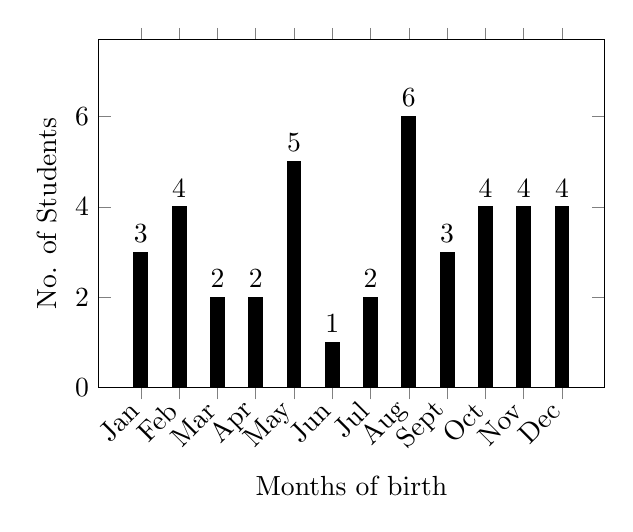
\begin{tikzpicture}
\begin{axis}[
ybar,
ymin=0,
width=8cm,
height=6cm,
ymax=7,
bar width=5pt,
ylabel={No. of Students},
xlabel={Months of birth},
nodes near coords,
symbolic x coords={Jan,Feb,Mar,Apr,May,Jun,Jul,Aug,Sept,Oct,Nov,Dec},
xtick = data,
x tick label style={rotate=45,anchor=east},
enlarge y limits={value=0.1,upper},
legend pos=north east,
],
\addplot[fill=black] coordinates {(Jan,3) (Feb,4)(Mar,2) (Apr,2)(May,5)(Jun,1)(Jul,2)(Aug,6)(Sept,3)(Oct,4)(Nov,4)(Dec,4)};
\end{axis}
\end{tikzpicture}\\

Observe the bar graph given above and answer the following questions:\\

(i) Many students were born in the month of November?\\
(ii)In which month were the maximum number of students born?\\

\item A family with a monthly income of \rupee 20,000 had planned the following
expenditures per month under various heads:\\
\begin{tabular}{|c|c|}
\hline
\textbf{Heads} &\textbf{Expenditure(in 1000\rupee)}\\
\hline
Grocery &4\\
Rent &5\\
Education of children &5\\
Medicine &2\\
Fuel &2\\
Entertainment &1\\
Miscellaneous &1\\
\hline
\end{tabular}\\

Draw a bar graph for the data above.\\

\item A teacher wanted to analyse the performance of two sections of students in a mathematics test of 100 marks. Looking at their performances, she found that a few students got under 20 marks and a few got 70 marks or above. So she decided to
group them into intervals of varying sizes as follows: 0 - 20, 20 - 30, . . ., 60 - 70, 70 - 100. Then she formed the following table:\\
\begin{tabular}{|c|c|}
\hline
\textbf{Marks} &\textbf{Number of students}\\
\hline
0-20 &7\\
20-30 &10\\
30-40 &10\\
40-50 &20\\
50-60 &20\\
60-70 &15\\
70-above &8\\
\hline
\textbf{Total} &90\\
\hline
\end{tabular}\\
\item Consider the marks, out of 100, obtained by 51 students of a class in a test, given in Table.\\
\begin{tabular}{|c|c|}
\hline
\textbf{Marks} &\textbf{No.of Students}\\
\hline

0-10 &5\\
10-20 &10\\
20-30 &4\\
30-40 &6\\
40-50 &7\\
50-60 &3\\
60-70 &2\\
70-80 &2\\
80-90 &3\\
90-100 &9\\
\hline
\textbf{Total} &51\\
\hline
\end{tabular}\\

Draw a frequency polygon corresponding to this frequency distribution table.\\

\item n a city, the weekly observations made in a study on the cost of living index are given in the following table:\\
\begin{tabular}{|c|c|}
\hline
\textbf{Cost of living index} &\textbf{No. of weeks}\\
\hline
140-150 &5\\
150-160 &10\\
160-170 &20\\
170-180 &9\\
180-190 &6\\
190-200 &2\\
\hline
\textbf{Total} &52\\
\hline
\end{tabular}\\

Draw a frequency polygon for the data above (without constructing a histogram).\\
\item 5 people were asked about the time in a week they spend in doing social work in their community. They said 10, 7, 13, 20 and 15 hours, respectively. Find the mean (or average) time in a week devoted by them for social work.\\
\item Find the mean of the marks obtained by 30 students of Class IX of a school, given below\\

\begin{tabular}{cccccccccc}
10 &20 &36 &92 &95 &40 &50 &56 &60 &70\\
92 &88 &80 &70 &72 &70 &36 &40 &36 &40\\
92 &40 &50 &50 &56 &60 &70 &60 &60 &80\\
\end{tabular}\\

\item The heights (in cm) of 9 students of a class are as follows:\\
155 160 145 149 150 147 152 144 148\\
Find the median of this data.\\
\item The points scored by a Kabaddi team in a series of matches are as follows:\\
17, 2, 7, 27, 15, 5, 14, 8, 10, 24, 48, 10, 8, 7, 18, 28 \\
Find the median of the points scored by the team.\\
\item Find the mode of the following marks (out of 10) obtained by 20 students:\\
4, 6, 5, 9, 3, 2, 7, 7, 6, 5, 4, 9, 10, 10, 3, 4, 7, 6, 9, 9\\
\item Consider a small unit of a factory where there are 5 employees : a supervisor and four labourers. The labourers draw a salary of \rupee 5,000 per month each while the supervisor gets \rupee 15,000 per month. Calculate the mean, median and mode
of the salaries of this unit of the factory.\\



